%%%%%%%%%%%%%%%%%%%%%%%%%%%%%%%%%%%%%%%%%%%%%%%%%%%%%%%%%%%%%%%%%%%%%%
%  月度总结 · 阶段二（研究推进）
%  控制算法方向
%
%  编译：xelatex 本文件（跑两遍）
%  Overleaf：Menu -> Compiler -> XeLaTeX
%%%%%%%%%%%%%%%%%%%%%%%%%%%%%%%%%%%%%%%%%%%%%%%%%%%%%%%%%%%%%%%%%%%%%%
\documentclass[stage2]{ydzjreport}

% ===================== 只改这里：你的信息 =====================
\stagetwosetup
  {阶段二 · 进阶阅读}%              1 报告阶段
  {张昊洋}%                         2 姓名
  {流量动态调控}%                    3 方向
  {2026-09-01 至 2026-09-30}%       4 报告周期
  {控制算法；增量式 PID；函数辨识；执行器特性}% 5 关键词
  {理清组长提出的控制实验，把「执行器→流速」「流速→芯片温度」
   确立为两个待辨识函数并给出叠加式建模方案；
   同时完成控制回路建模与增量式 PID 的仿真验证。}% 6 一句话摘要
% ============================================================

\begin{document}
\makestagetwohead

% ==================================================================
\section{本月研究任务}

\subsection{任务目标}

\begin{enumerate}
  \item 把组长提出的控制实验整理成可执行的方案，明确变量角色与待辨识对象；
  \item 完成控制回路的数学建模与基础 PID 控制器的仿真验证；
  \item 判断是否需要引入智能算法（强化学习），并给出依据。
\end{enumerate}

\subsection{完成情况}

\begin{table}[htbp]
\centering
\caption{本月任务完成情况}
\begin{tabularx}{\textwidth}{@{}Y c Y@{}}
\toprule
\rowcolor{ydzjlight} 任务 & 状态 & 说明 \\
\midrule
控制实验方案整理 & 已完成 & 变量角色与两个待辨识函数已明确，方案待组长确认 \\
控制回路建模 & 已完成 & 一阶热平衡模型，含执行器非线性映射 \\
基础 PID 仿真验证 & 已完成 & 增量式 PID，含积分限幅与输出限幅 \\
二阶对象动态特性分析 & 已完成 & 阻尼比与固有频率的参数扫描 \\
智能算法可行性判断 & 已完成 & 结论：现阶段不引入 DRL，理由见 §\ref{sec:qishi} \\
执行器/散热片实测辨识 & 未开始 & 缺实验条件，见 §\ref{sec:que} \\
\bottomrule
\end{tabularx}
\end{table}

% ==================================================================
\section{进阶阅读与理论支撑}

\subsection{本阶段文献清单}

\begin{table}[htbp]
\centering
\caption{本阶段文献及其针对性}
\begin{tabularx}{\textwidth}{@{}c Y Y@{}}
\toprule
\rowcolor{ydzjlight} 序号 & 文献 & 解决了我哪个问题 \\
\midrule
1 & Vignon 等, 2023, DRL 用于流动控制的进展与展望 & 判断 DRL 是否该作为本项目主线 \\
2 & Brunton \& Kutz, 2022, 数据驱动科学与工程 & 系统辨识需要哪些前置条件、实验怎么设计 \\
3 & 陶飞等, 2024, 数字孪生的发展与挑战 & 「物理模型 + 数据修正」的落地路径 \\
\bottomrule
\end{tabularx}
\end{table}

\subsection{对本方向的启示}
\label{sec:qishi}

原本我打算在 PID 之上直接叠加 DRL。读完这三篇后改成了\textbf{「先辨识、后控制、暂不上 DRL」}，理由有三。

\textbf{第一，改的是顺序而不是算法。} Brunton 明确指出系统辨识是数据驱动控制的前置步骤——没有可信的对象模型，任何控制器的评价都缺乏基准。这正好解释了为什么组长要求先做控制实验：不是走流程，而是控制算法无法凭空设计。

\textbf{第二，改的是对 DRL 的定位。} 我原来把 DRL 当作「更高级的 PID」，读完后认识到它是\textbf{需要大量交互样本的决策算法}。我们目前只有仿真环境，样本来自 CFD 而非实物，训练出的策略迁移到真实台架上有明显风险。

\textbf{第三，改的是技术路线。} 陶飞强调数字孪生需要物理模型与实测数据\emph{双向校准}。因此把路线定为：一阶物理模型打底 → 实测数据辨识参数 → 经典控制先行 → 视数据积累情况再评估学习型控制。这条路线更慢但更稳。

% ==================================================================
\section{研究进展}

\subsection{已完成的工作}

\begin{enumerate}
  \item \textbf{梳理控制实验的变量结构。} 把系统整理为三条链：
        \[
        \underbrace{P,\,V}_{\text{执行器}}
        \;\xrightarrow{\;f\;}\;
        \underbrace{Q}_{\text{流速}}
        \;\xrightarrow{\;g\;}\;
        \underbrace{T_c}_{\text{芯片温度}}
        \]
        其中 $P$ 为泵转速、$V$ 为阀开度（未来加装）、$Q$ 为流速、$T_c$ 为芯片温度；
        入口水温 $T_{in}$ 为另一自变量，热流密度 $q$ 为不可控扰动。
        \textbf{待辨识的是 $f$ 与 $g$ 两个函数。}变量结构见 图~\ref{fig:block2}。
\begin{figure}[htbp]
\centering
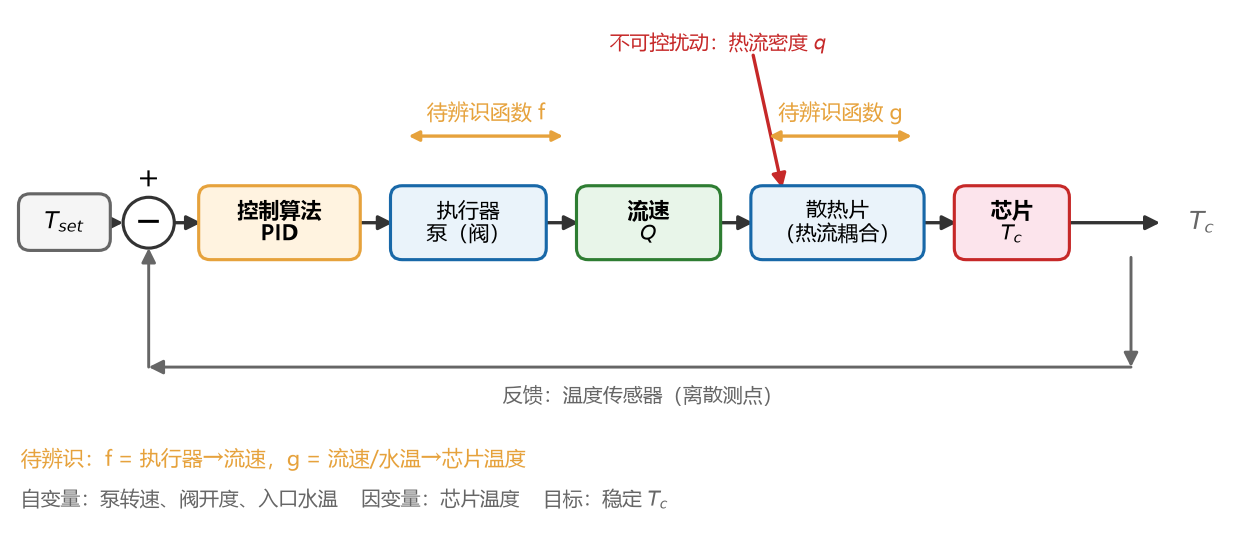
\includegraphics[width=0.92\textwidth]{figs/fig_block.png}
\caption{控制系统的变量结构与待辨识的两个函数}
\label{fig:block2}
\end{figure}


  \item \textbf{建立一阶热平衡模型。} 将「热源—散热片—冷却液」简化为集总参数模型：
        \[
        \frac{\mathrm{d}T}{\mathrm{d}t}
        = a\,(T_{heat}-T) - k(u)\,(T-T_{amb}) - b\,(T-T_{amb})
        \]
        其中 $u$ 为执行器开度，$k(u)$ 为开度到散热能力的非线性映射，暂用幂次经验式
        $k(u) = k_{min} + (k_{max}-k_{min})(u/100)^{0.8}$。

  \item \textbf{实现增量式 PID 控制器}，并加入两重工程约束：
        积分限幅 $\text{integral}\in[-100,100]$ 抑制积分饱和；
        输出限幅 $u\in[0,100]$ 对应执行器实际行程。

  \item \textbf{完成二阶对象动态特性分析}（复现详见阶段一报告）。
\end{enumerate}

\subsection{关键结果}

\begin{table}[htbp]
\centering
\caption{仿真工况与控制器参数}
\begin{tabularx}{\textwidth}{@{}Y Y@{}}
\toprule
\rowcolor{ydzjlight} 项目 & 取值 \\
\midrule
目标温度 & 68 \textcelsius \\
热源基础温度 / 波动幅度 & 82 \textcelsius\ / $\pm$12 \textcelsius \\
热源波动周期 & 15 s（可调 5--30 s） \\
初始温度 / 环境温度 & 50 \textcelsius\ / 25 \textcelsius \\
PID 参数 & $K_p = 8.0$，$K_i = 0.5$，$K_d = 2.0$ \\
控制周期 & 50 ms \\
加热系数 $a$ & 0.45 \\
执行器散热系数范围 & $k_{min}=0.03$（全关）$\sim k_{max}=0.20$（全开） \\
\bottomrule
\end{tabularx}
\end{table}

\begin{table}[htbp]
\centering
\caption{二阶对象性能指标（$\omega_n = 1$ rad/s，理论值与仿真一致）}
\begin{tabularx}{\textwidth}{@{}c c c c c@{}}
\toprule
\rowcolor{ydzjlight} 阻尼比 $\zeta$ & 超调量 & 峰值时间 /s & 上升时间 /s & 调节时间 /s \\
\midrule
0.3   & 37.23\% & 3.293 & 1.966 & 13.33 \\
0.5   & 16.30\% & 3.628 & 2.418 & 8.00 \\
0.707 & 4.33\%  & 4.442 & 3.331 & 5.66 \\
1.0   & 0       & --- & --- & 4.00 \\
\bottomrule
\end{tabularx}
\end{table}

\textbf{说明}：上表为\emph{对象自身}的动态特性，用于确定控制器应有的响应速度；它不是控制器闭环性能，后者需在接入辨识模型后重新评估。控制器闭环的仿真时程见 图~\ref{fig:pidsim}。

上述工况下的闭环仿真结果汇总于 表~\ref{tab:simres}。

\begin{table}[htbp]
\centering
\caption{闭环仿真结果（对应 图~\ref{fig:pidsim}）}
\label{tab:simres}
\begin{tabularx}{\textwidth}{@{}Y c Y@{}}
\toprule
\rowcolor{ydzjlight} 指标 & 数值 & 说明 \\
\midrule
芯片温度范围 & 50.7 $\sim$ 72.1 \textcelsius & 含启动阶段的爬升过程 \\
稳态平均温度 & 68.7 \textcelsius & 后半程均值，与目标 68 \textcelsius\ 相差 0.7 \textcelsius \\
峰值超调 & $+$3.9 \textcelsius（5.7\%） & 相对目标温度 \\
阀开度范围 & 0 $\sim$ 100\% & \textbf{触及两端行程} \\
阀开度均值 & 54.4\% & 说明执行器工作在可用行程中部 \\
上行程饱和时间占比 & 29.3\% & 开度已达 100\% 仍无法降温的时段 \\
下行程饱和时间占比 & 16.7\% & 开度已关到 0 的时段 \\
积分项峰值 & 100（已被限幅） & 未限幅时可达 1052.6 \\
\bottomrule
\end{tabularx}
\end{table}
\begin{figure}[htbp]
\centering
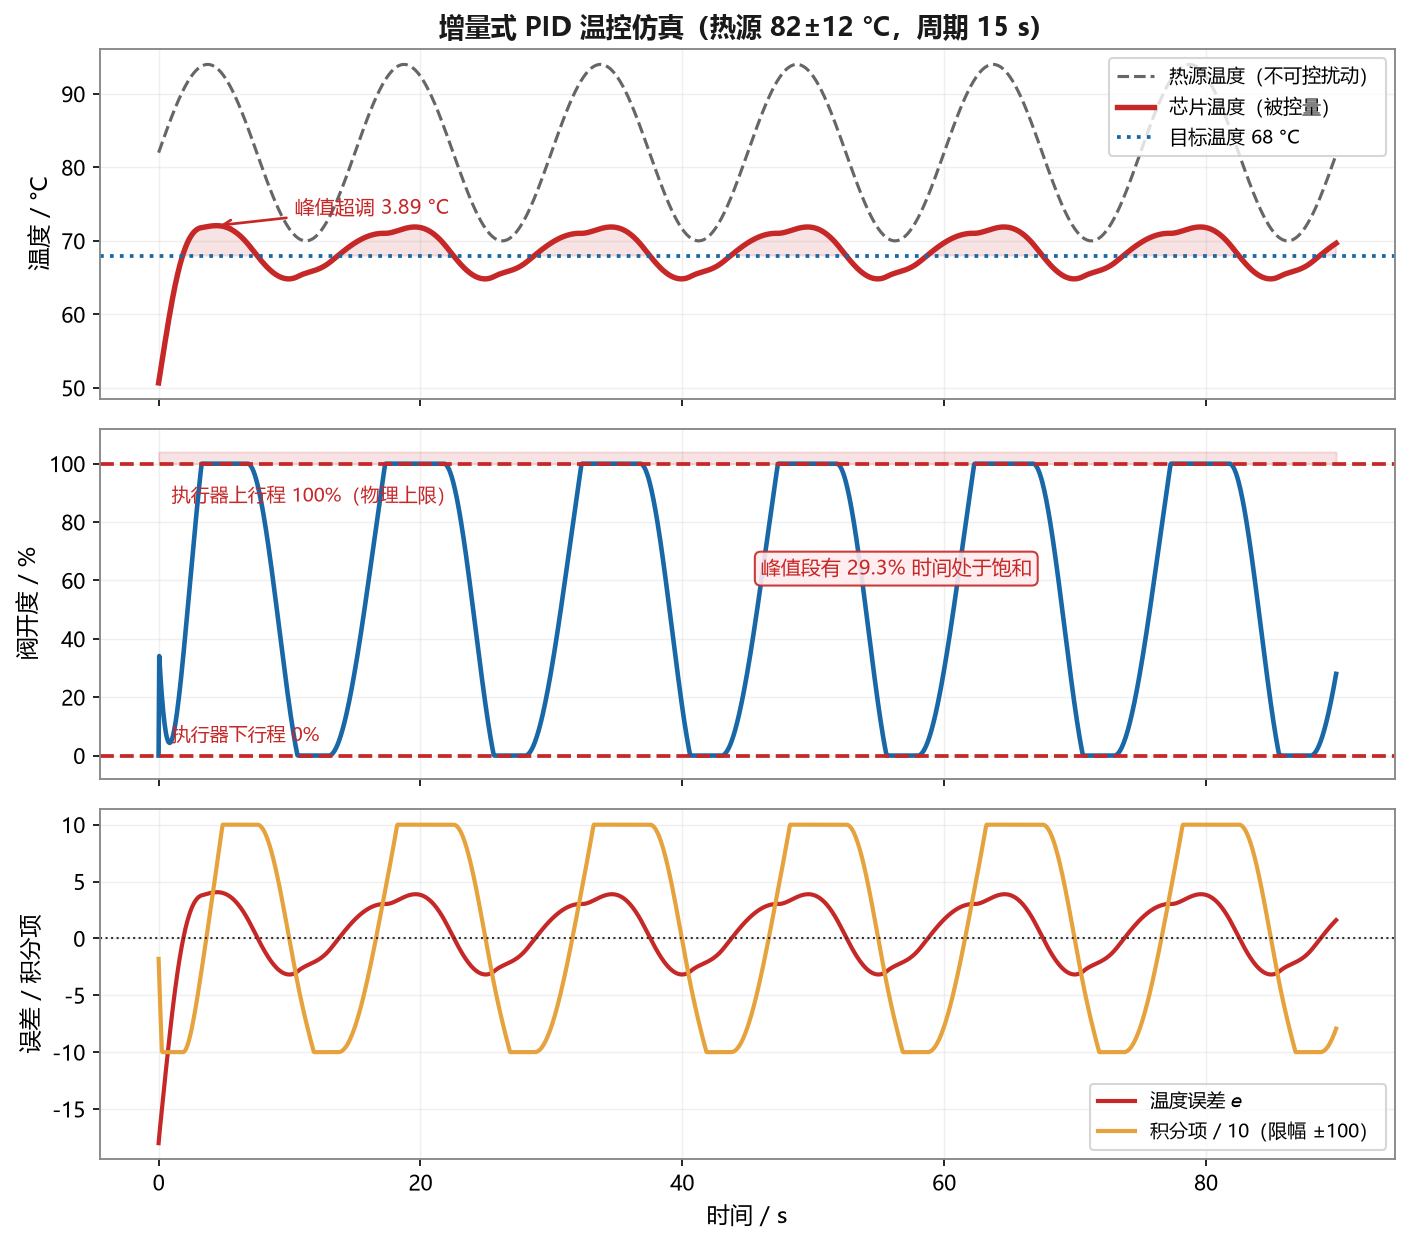
\includegraphics[width=0.70\textwidth]{figs/fig_pid_sim.png}
\caption{增量式 PID 温控仿真时程：温度、阀开度与误差/积分项}
\label{fig:pidsim}
\end{figure}


\subsection{与预期的差异}

\textbf{预期}：增量式 PID 加入积分限幅后，应能消除积分饱和引起的超调。

\textbf{实际}：限幅确实把积分项从 \textbf{1052.6 压到了 100}（见表~\ref{tab:simres}），但\textbf{超调并未消失，只是从「持续增大」变成了「有上界」}——峰值仍有 $+$3.9 \textcelsius（5.7\%）。把误差、积分项、阀开度三条曲线叠在一起观察（图~\ref{fig:pidsim}）后发现：根本原因不是积分饱和，而是\textbf{执行器的散热能力存在物理上限}。仿真中有 \textbf{29.3\% 的时间阀开度已达 100\%}，此时误差仍为正，无论控制器输出什么都不会有效果，温度必然继续上升，形成结构性超调。

\textbf{这个差异改变了我的下一步方向}：不是继续在 PID 参数与抗饱和上做文章，而是\textbf{必须先把执行器的实际能力边界测出来}。如果台架上泵的最大流量不足以应对峰值热流，那这是选型问题而非算法问题。这也再次指向组长要求的控制实验。

% ==================================================================
\section{问题与对策}

\subsection{遇到的主要问题}

\begin{enumerate}
  \item \textbf{执行器特性完全未知。} 现有模型中 $k(u)$ 是我凭经验设定的幂次式，没有任何实测依据；泵转速与流速的真实关系也不清楚。参数不可信，仿真结论就只能定性。
  \item \textbf{未来要加装水阀，双执行器的耦合关系不明。} 关小阀门会改变管路阻力，进而影响泵的工作点。若耦合显著，两个执行器就不能当独立变量处理。
  \item \textbf{温度测点与控制目标不一致。} 控制要稳定的是芯片\emph{最高}温度，而传感器只能给出若干离散测点温度，二者之间的偏差没有量化依据。
\end{enumerate}

\subsection{已尝试的方案}

\begin{enumerate}
  \item 针对问题 1，尝试用已有的 CFD 结果反推散热能力——但 CFD 给出的是稳态场，缺少\emph{动态}响应信息，无法直接得到 $k(u)$ 的时变特性，只能给出稳态趋势。
  \item 针对问题 2，尝试用「固定阀门、只调泵」的简化方式回避耦合——这样虽然能先跑通控制器，但一旦加装水阀就需要重做，属于暂时回避而非解决。
  \item 针对问题 3，尝试用测点平均温度作为控制目标——平均温度会掩盖热点，与「防止芯片过热」的目标不符，暂不采用。
\end{enumerate}

\subsection{下一步对策}

\begin{enumerate}
  \item \textbf{设计并执行辨识实验}，用增量叠加形式降低实验量（方案见 §\ref{sec:plan} 与 表~\ref{tab:ident}）。
  \item \textbf{在加装水阀前先用单执行器完成标定}，把泵的特性曲线测准；水阀到位后只需补测耦合项，不必重做全部工作。
  \item \textbf{把控制目标改为「测点最高温不超过阈值」}，而不是「平均温度稳定在某值」。这样即使测点与真实热点有偏差，也属于偏保守的方向，安全性更好。
\end{enumerate}

% ==================================================================
\section{阶段性结论}

\subsection{可以确定的}

\begin{enumerate}
  \item \textbf{控制回路的基本逻辑是正确的。} 仿真中温度偏高则增大开度、偏低则减小，方向始终正确，未出现反向调节。
  \item \textbf{增量式 PID 的两重限幅是必要的。} 积分限幅与输出限幅均按预期动作，避免了输出越界这类最危险的情况。
  \item \textbf{智能算法现阶段不应作为主线。} 依据是数据需求与实测条件的双重不匹配，而非算法本身不好；后续若实验数据充足，可以重新评估。
  \item \textbf{必须先辨识、后控制。} 这一点已由本月「超调并非源于积分饱和」的分析得到印证——对象与执行器不清楚时，调参是在猜。
\end{enumerate}

\subsection{尚不能确定的}
\label{sec:que}

\begin{enumerate}
  \item \textbf{执行器的能力边界。} 泵的最大流量、最小可调流量，以及未来水阀的分辨率，都需实测才能确定。若最大流量不足以带走峰值热流，则需更换选型，这会改变整个控制方案的前提。
  \item \textbf{两个执行器的耦合程度。} 泵与阀之间是否可近似解耦，决定了后续用单变量控制还是多变量控制。缺的实验证据是：固定泵转速、改变阀开度时，观察泵的工作点是否移动。
  \item \textbf{控制通道的时间尺度。} 从改变泵转速到芯片温度出现可测变化，这个延迟到底是零点几秒还是几十秒，直接决定控制周期与控制策略的选择。目前仿真中用的时间常数是假定值。调节时间与阻尼比的关系见 图~\ref{fig:metrics2}。
\begin{figure}[htbp]
\centering
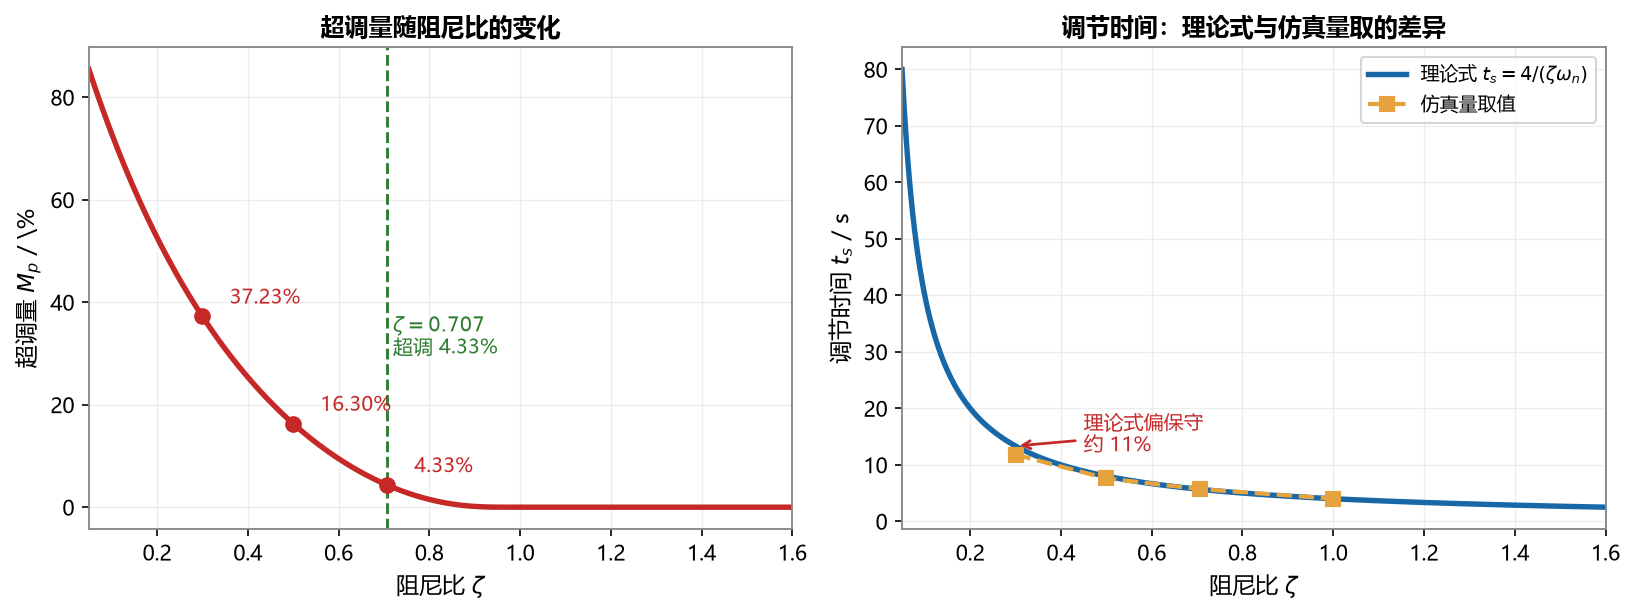
\includegraphics[width=0.98\textwidth]{figs/fig_metrics.png}
\caption{调节时间随阻尼比的变化：理论式与仿真量取的差异}
\label{fig:metrics2}
\end{figure}

\end{enumerate}

% ==================================================================
\section{下月计划}
\label{sec:plan}

\begin{table}[htbp]
\centering
\caption{两个待辨识函数与对应的实验设计}
\label{tab:ident}
\begin{tabularx}{\textwidth}{@{}c Y Y Y@{}}
\toprule
\rowcolor{ydzjlight} 序号 & 待辨识对象 & 实验方法 & 预期产出 \\
\midrule
1 & $Q = f(P,V)$：泵转速与阀开度对流速的影响
  & 固定阀开度扫泵转速；固定泵转速扫阀开度；再取少量泵阀组合验证耦合项
  & 泵特性曲线、阀特性曲线、耦合系数 \\
2 & $T_c = g(Q,T_{in},q)$：流速与水温对芯片温度的影响
  & 固定热流密度，扫流速；固定流速，扫入口水温；再改变热流密度验证
  & 稳态增益 $k_Q$、$k_T$、$k_q$ 与时间常数 \\
\bottomrule
\end{tabularx}
\end{table}

\begin{table}[htbp]
\centering
\caption{下月工作计划}
\begin{tabularx}{\textwidth}{@{}Y Y c@{}}
\toprule
\rowcolor{ydzjlight} 事项 & 预期产出 & 时间 \\
\midrule
向组长确认实验条件（泵型号、是否已有阀、可测量的量） & 实验条件清单 & 第 1 周 \\
细化辨识方案（测点布置、采样频率、工况点选取） & 辨识实验细则 & 第 1--2 周 \\
在现有仿真环境预演辨识流程，验证方法可行 & 预演结果与误差评估 & 第 2--3 周 \\
整理控制部分已有模型与代码，形成方法文档 & 可复现代码 + 方法说明 & 第 3--4 周 \\
\bottomrule
\end{tabularx}
\end{table}

\begin{notebox}
\textbf{关于水阀的说明}：水阀为\emph{未来计划加装}，现有系统尚无此执行器。因此本月的方案设计按「泵为主执行器」展开，并预留了水阀接入后的耦合项补测环节，避免加装后需要重做全部标定。
\end{notebox}

% ==================================================================
\begin{thebibliography}{9}
\bibitem{vignon23} VIGNON C, RABAULT J, VINUESA R. Recent advances in applying deep reinforcement learning for flow control: Perspectives and future directions[J]. Physics of Fluids, 2023, 35(3): 031301.
\bibitem{brunton22} BRUNTON S L, KUTZ J N. Data-driven science and engineering: Machine learning, dynamical systems, and control[M]. 2nd ed. Cambridge: Cambridge University Press, 2022.
\bibitem{tao24} TAO F, ZHANG H, ZHANG C. Advancements and challenges of digital twins in industry[J]. Nature Computational Science, 2024, 4(3): 169-177.
\end{thebibliography}

\end{document}
